%pæn (projekttitel på forside!!!)
%vi skal også beskrive interne regler (fx bødekasse)
%sekvensdiagram
%designmockups


\documentclass[11pt,a4paper]{report}

\setlength{\textwidth}{165mm}
\setlength{\textheight}{240mm}
\setlength{\parindent}{0mm} % S{\aa} meget rykkes ind efter afsnit
\setlength{\parskip}{\baselineskip}
\setlength{\headheight}{0mm}
\setlength{\headsep}{0mm}
\setlength{\hoffset}{-2.5mm}
\setlength{\voffset}{0mm}
\setlength{\footskip}{15mm}
\setlength{\oddsidemargin}{0mm}
\setlength{\topmargin}{0mm}
\setlength{\evensidemargin}{0mm}




\usepackage{courier} % The font we use.
\usepackage[a4paper, hmargin={2.8cm, 2.8cm}, vmargin={2.5cm, 2.5cm}]{geometry}
\usepackage{eso-pic} % \AddToShipoutPicture
\usepackage{graphicx} % \includegraphics
\usepackage[english]{babel}
\usepackage[utf8]{inputenc}
\usepackage{appendix}
\usepackage{amsfonts,amsmath,amssymb}
\usepackage[colorinlistoftodos]{todonotes}
%\usepackage{gauss} % Gauss Matrix
\usepackage{float} % This will allow precise picture placement, use [H].
\usepackage{enumitem}



\usepackage{microtype}
\usepackage[super]{nth}
\usepackage{booktabs} % This package provide some additional commands to enhance the quality of tables in LaTeX.
\usepackage{listings} % code parsing.
\PassOptionsToPackage{hyphens}{url}\usepackage{hyperref}
\lstset{language=bash} % Set bash syntax.

\newcommand{\code}[1]{\texttt{#1}}

\newlist{SubItemList}{itemize}{1}
\setlist[SubItemList]{label={$-$}}

\let\OldItem\item
\newcommand{\SubItemStart}[1]{%
    \let\item\SubItemEnd
    \begin{SubItemList}[resume]%
        \OldItem #1%
}
\newcommand{\SubItemMiddle}[1]{%
    \OldItem #1%
}
\newcommand{\SubItemEnd}[1]{%
    \end{SubItemList}%
    \let\item\OldItem
    \item #1%
}
\newcommand*{\SubItem}[1]{%
    \let\SubItem\SubItemMiddle%
    \SubItemStart{#1}%
}%

\newcommand{\BAR}{%
  \hspace{-\arraycolsep}%
  \strut\vrule % the `\vrule` is as high and deep as a strut
  \hspace{-\arraycolsep}%
}


\author{\Large{Sven Frenzel (\href{mailto:sven@frenzel.dk}{sven@frenzel.dk}) - 130793 - cdn769}\\
\Large{Mads Gram (\href{mailto:mgmadsgram@gmail.com}{mgmadsgram@gmail.com})  - 081293 - wtc324}\\
\Large{Thorkil Værge (\href{mailto:thorkilk@gmail.com}{thorkilk@gmail.com}) - 150287 - wng750} \\ \\
\Large{Instructor: Kasper Passov }}

\title{
\vspace{3cm}
\Large{\nth{4} Partial Assignment -- ProjDat}
}

\begin{document}

%% Change `ku-farve` to `nat-farve` to use SCIENCE's old colors or
%% `natbio-farve` to use SCIENCE's new colors and logo.
\AddToShipoutPicture*{\put(0,0){\includegraphics*[viewport=0 0 700 600]{include/natbio-farve}}}
\AddToShipoutPicture*{\put(0,602){\includegraphics*[viewport=0 600 700 1600]{include/natbio-farve}}}

%% Change `ku-en` to `nat-en` to use the `Faculty of Science` header
\AddToShipoutPicture*{\put(0,0){\includegraphics*{include/nat-en}}}

\clearpage\maketitle
\thispagestyle{empty}

\newpage
\tableofcontents{}
\thispagestyle{empty}


\newpage

\chapter{Literature Review}\label{ch:Literature_Review}


\section{Highsmith J. - Extreme Programming}
\subsection{Résumé}

The article points out that the price tag of the development of a program through its life cycle is skewed towards the back end, meaning that the majority of resources (money) is spent on maintenance. It thus criticizes older methodologies while promoting a more minimal design strategy. This, more minimal design strategy seeks to unskew the cost of the life cycle such that it becomes more uniform. The change in cost of maintenance will warrant a shift in the balance of design and refactoring, reducing the focus from creating large systems, in which system architects try to anticipate the inevitable changes. These new methodologies will enable rapid changes to the system, allowing refactoring such that features can be added to the system, without the need of a total remodeling of the entire system.

Extreme Programming is mentioned as the main contender to solve the problem in question, but other Lean development methodologies are also mentioned and compared.

\subsection{Extreme Programming (XP)}

To face the challenges of a contemporary market, where continuous change is a reality, Highsmith introduces the methodology of Extreme Programming (XP).
For XP to solve the problems of continuous change, XP employs a set of practices. These serve as guidelines for the development team. Rather than demanding all practices to be followed, a focus on choosing practices that aid the development is emphasized. But some guidelines are interdependent so they cannot be chosen arbitrarily. A few examples of these practices are: pair programming, simple design and refactoring. When the practices of XP are employed together, the process of system development aligns towards the core values of XP. XP is represented as a methodology that primarily is applicable to small teams.


\subsection{Refactoring}
Throughout the article, one of the main elements is both represented as an idea and a practice for the mentioned methodologies. Refactoring is introduced as an aspect which both builds new functionally into a system, but also mends or improves the current internal structure of the code base.

\subsection{Analysis and Perspective}
In the contemporary world we often see new services appearing. Not all of these are successful, but sometimes a new service that reshapes a market arises. Services such as Facebook have altered social media, and forced many services to adapt: For example, log ins to post a comment on a news site can often be done through Facebook.

The idea of continuously having to adapt to a market that is poised to change, aligns perfectly with the methodology of Extreme Programming.

\subsection{Perspectivation to Work on DIKU Keys}
We have, to some degree, utilized pair programming when the web application was set up to communicate with the email server. This was a good way of working since both users were new to Golang and it was nice to have some moral and practical support.

The relevant theory from this paper that we can extract regarding DIKU Keys is that the code should be easily maintainable such that it can respond to changing needs. However, a university computer system does not live in a very competitive environment since there is virtually no competition. The computer systems are chosen through centralized decision making and not by its end-users.

\section{Naur, P. (1985) Programming as Theory Building}
\subsection{Résumé}
Programming as Theory Building presents a paradigm to understand the process of software engineering in which the main process of the programming task is not the production of documents and code but the acquirement of knowledge and theoretical understanding of a system. A system is here considered both the real world objects which the system maps and the actual server/computer and software running the service. The paper is a presentation of the theory and not a full endorsement in the sense that Naur explains what the theory suggests and criticizes some of its conclusions while supporting other.

Programming as Theory Building is contrasted to a production view where programmers are viewed as a kind of factory worker who follow formalized rules and can easily be exchanged. The theory paradigm can, unlike the production paradigm, explain why it is so hard to modify or maintain a given system if it is done by programmers without prior knowledge of the system. As an example of the importance of theoretical understanding of the system that a programmer works on, Naur presents two cases where some programmers have modified a programming language (the lexers, parsers, etc.) invented by some other people. The documentation of the code was provided to both groups but the support and guidance was only provided to one group. In the case where the new developers had access to the original developers, the modification relied heavily on the knowledge of the original (language inventors) group. In the case where the original developers did not provide support or help, the result was not aligned with the spirit of the original language; it was a clumsy implementation. This further suggest that the theory that is acquired by the programmers is not only essential for the production of good software but also tacit -- which means that it cannot be fully captured in words but must be learned through experience.

Naur suggests that the experience of general programming models can be taught by model problems and solutions which extend the tacit knowledge of the programmer.

The role of rules and models in programming is discussed and it is stated that intuition and experience take primacy over rules since experience and intuition determines which rules and programming models that should be followed.

The importance of theoretical knowledge of a system leads to the categorization of programs into three states: ``Alive'', where the theoretical knowledge of the program is present in developers; ``dead'', the theory is gone; and revived, the knowledge is being reinvented. But Naur actually suggests that a program cannot be revived but can only be reinvented/rewritten/remade since the original theory cannot be acquired without the help of the original programmers. If the theory of a program is gone, the program should be remade and not revived.

Naur draws two further conclusions:
\begin{itemize}
\item The theory view of the programming task should raise the status of the programmers in companies from one of production workers to that of lawyers or managers.
\item The theory view necessitates that computer science students should learn to acquire knowledge of systems and the real-world objects that it maps. Whether this is possible, is an open question but should be attempted through project courses in computer systems design, where the students are under the competent guidance of wise and benevolent teachers ...
\end{itemize}
\subsection{Analysis and Perspective}
The quality differences in the cases where a programming language is extended, are not proved. So the quality differences that Naur describes could be attributable to subjective valuations and not objective facts and the paper would have made a stronger case in this regard if it had been able to back up this claim.

In our opinion, the article presents a false dichotomy between the production view and the theory view. The production paradigm articles that we have encountered did in no way rule out that the main motivation behind the production of various models was to acquire theoretical knowledge of the program. This means that the main benefit of designing a system according to the rational design model\cite{art:parnas} might very well be the acquirement of theory amongst the programmers but that the best way to acquire this theory is to follow the rational design process. So the paradigms might have different foci but are not necessarily mutually exclusive in the actual work process.

The theory paradigm does however excel in explaining why system maintenance should be done by the original programmers and is a very hard, or impossible task, if the theory is not present in the new programming group.
\subsection{Perspectivation to Work on DIKU Keys}
The work on DIKU Keys has to a large extent been about producing material such as class diagrams, sequence diagrams, initial software architecture, and BCE models. A prerequisite for the production of this material was to understand the content and the theory of for example a class diagram. So the production requirements are directly responsible for the acquirement of theoretical understanding. This supports the idea that there is no dichotomy between the production requirements (or production focus) and the Theory Building.

This means that this article is theoretically interesting and may explain some things and warn against for example the destruction of knowledge in companies, but in the actual programming and design phase it is irrelevant since a focus on the production requirements automatically builds the required theory.


\chapter{Project Report}\label{ch:Project_Report}

\section{Abstract}\label{sec:Abstract}
The system developed [system], as part of this project, is a module of a system developed by Oleksander Shturmov [Online TA]. The purpose of the system is to validate the identity of a student submitting an assignment to Online TA. \\
This is done by mapping OpenPGP keys provided by the students with their KU ID. This mapping is achieved through a website on which a student registers themselves. The website is part of the system developed. Furthermore an API is provided to Online TA for integration. The system is developed for the Department of Computer Science at the University of Copenhagen [DIKU] represented by Oleksander Shturmov. Oleksander Shturmov has shown a desire to replace the currently used Learning Management System [LMS] \textit{its Learning} with a platform that can facilitate automatically evaluation of programming assignments. For this he requires a system to make sure that a given assignment has been handed in by the student claiming to have handed it in. This is the system we are developing.
A prototype of the system is available at \url{http://dikukeys.dk}.

\section{Purpose and Framework for the Project}\label{sec:Purpose_Framework}
This definition is based on the FACTOR criteria\cite{book:factor} which serves the purpose of providing the structure for a systems definition.
\begin{itemize}
\item \textbf{F}unctionality: The purpose of the system is to allow specific students and employees\footnote{Everyone with valid KU ID in the form of xyz123 - 'svensk nummberplade'.} at the University of Copenhagen to map their username to a public PGP key and store these records in a database maintained by the customer. The system must also allow the same users to replace their public key in case they lose the corresponding private key. The mappings should be readable by specific users with privileged access through some login mechanism.
There should also exist an automatic way for other systems to access the mappings in a structured manner.
\item \textbf{A}pplication domain: The system will be used by students to upload their OpenPGP key and by teaching assistants to match hand-ins that have been signed by a student's OpenPGP key with a KU ID. It is used when TAs receive hand-ins by the students and before the grading commences.
\item \textbf{C}onditions: Most students are not likely to have experience with OpenPGP so it should be as simple as possible to upload a key and the system must be forgiving, meaning that if a student loses their private PGP key, they must be able to upload a new public key. Instructions to guide the students through the various tasks of creating and uploading a key must be available. The system must allow other software to access the mappings.
\item \textbf{T}echnology: Servers with a UNIX-like OS will run the system, and modern browsers will be used to display the front-end. The system will be written in golang to the widest extent possible but will also utilize SQL, HTML, CSS, and JS. It will also use existing software in the form of nginx for the http-server and existing golang libraries for example sqlite3.
\item \textbf{O}bjects: The primary objects in the problem domain are students, TAs, their KU ID, and public OpenPGP keys.
\item \textbf{R}esponsibility: The system's main responsiblity is to maintain a table with a mapping from KU IDs to corresponding OpenPGP public keys. It must also allow other privileged software and privileged users to read from this table.
\end{itemize}

\renewcommand{\thesubsection}{\thesection.\alph{subsection}}
\section{Specification of Requirements for the IT Solution}\label{sec:Requirements}
\subsection{Functional and Non-Functional Requirements}
\subsubsection{Functional Requirements}\label{subsubsec:Functional_Req}
The functional requirements describe features which are essential to the success of the project and describe actual functionality for the end-user or system administrator.
\begin{itemize}
\item The system must map a KU ID to an OpenPGP public key.
\item Users must be able to upload their own public key to the service.
\item If a user loses their private key, a method for replacing the public key must exist.
\item The initial registration of a key, and the replacement of a key, is authenticated through the KU email system.
\item The data has to be accessible to privileged software through a defined API.
\item The mappings have to be available to privileged users through some means.
\item The KU IDs registered in this system must \textbf{not} be accessible for non-privileged users and software.
\item A guide for creating key pairs needs to be available on the website, possibly as shell script. This guide should also explain how to use an OpenPGP key for SSH authentication.
\item A way for an administrator to send email invitations for joining the system to a list of students must exist.
\end{itemize}

\subsubsection{Non-functional Requirements}\label{subsubsec:Non_Functional_Req}
Non-functional requirements are system requirements which do not describe the actual functionality but instead describe either non-essential systems, internal architecture, or design.
\begin{itemize}
\item The back-end should be written in golang.
\item The front-end should be Javascript and HTML5.
\item The system must be browser independent\footnote{This includes recent versions of Internet Explorer, Chrome, Safari and Firefox.}.
\item The system must be compliant with all standards and regulations imposed by the Government of Denmark and the University of Copenhagen. These regulations concern privacy and restriction of access to the KU IDs that are part of the system. Specifically, the KU IDs in the system must not be accessible to non-privileged users\footnote{The privileged users are system administrators, university professors, and TAs.}.
\item The customer has decreed that the software be licensed under an MIT-like license which will be provided by the customer
\footnote{A preliminary version of this license is available on \href{https://github.com/oleks/sandstone/blob/master/LICENSE}{GitHub}.}.
\item The system should be able to decode the different .csv-formats (comma, semicolon, tab) for student lists.
\item The front-end must be responsive in its layout. This is achieved by using Bootstrap\footnote{Bootstrap can be found on \href{http://getbootstrap.com/}{http://getbootstrap.com/}}.
\item Kyoto Cabinet should be used as database management system \footnote{\href{http://fallabs.com/kyotocabinet/}{http://fallabs.com/kyotocabinet/}}
\end{itemize}

\subsection{Use Case Overview Model}\label{subsec:Use_case_model}

Figure \ref{fig:use_case_diagram_high_level} represents a high-level model which shows which actions are available for the different users: students and teachers. A student can upload and replace their public key and the TA can read the mappings. These are all the use cases that we have identified. They are the primary interactions between users and the system.

An API access to the system database has also been discussed but no clear specifications for this have been provided. Therefore that use case is not presented here.

\begin{figure}[H]
\centering
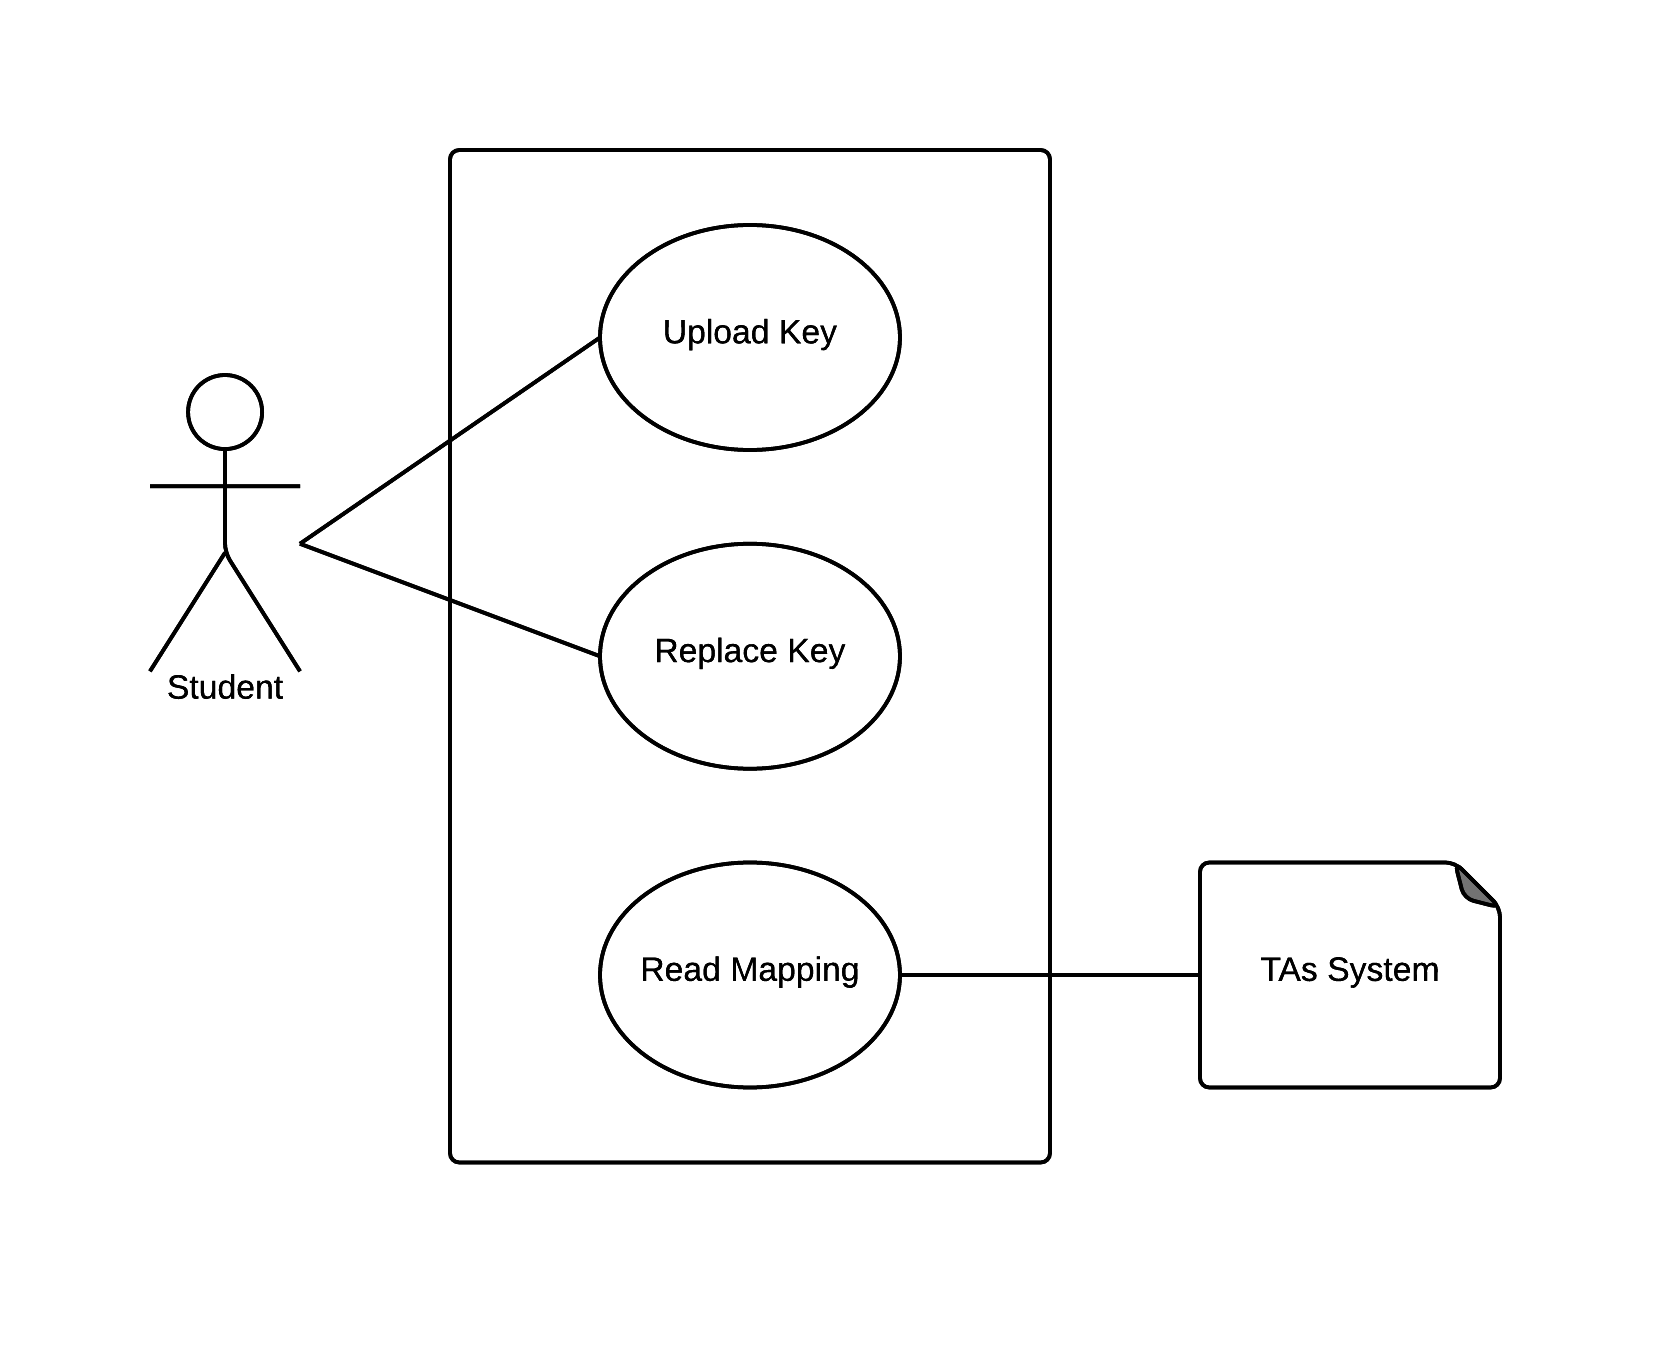
\includegraphics[width=0.5\textwidth]{pictures/use_case_pksu_del2_b_high}
\caption{High-level use case diagram. Students can upload or replace a public key, and teachers (TAs, professors, and system administrators) can pull data from the lists.}
\label{fig:use_case_diagram_high_level}
\end{figure}


\subsection{Specific Use Case Models}\label{subsec:Specific_Use_case_model}
Here, three different use cases for the system is shown by listing the actions of the relevant actors. The use cases for uploading a key, replacing a key, and sending out an invitation for joining the system are listed.
\subsubsection{Use Case: Upload Key}
\begin{tabular}{l p{0.77\textwidth}}
    \toprule
    \textit{Use case name} & Upload Key \\
    \midrule
    \textit{Participating} & Students \\
    \textit{actors} & \\
    \midrule
    \textit{Flow of events} &
    \vspace{-6.7mm} \begin{enumerate}
        \item Student follows link to dikukeys.dk in invitation email OR student goes to dikukeys.dk directly.
        \item Student enters their KU ID into a form.
        \item Server sends activation email to student's KU email address.
        \item Student follows link in activation email.
        \item Student posts their public key into a form or generates a key pair in the browser.
        \item Server sends email which confirms that a key has been uploaded.
    \end{enumerate}
    \\
    \midrule
    \textit{Entry condition} & User has an active KU ID. \\
                             & User is not registered in the system. \\
    \midrule
    \textit{Exit conditions} & User is registered in the system with a public key. \\
    \bottomrule
\end{tabular}

\subsubsection{Use Case: Replace Key}
\begin{tabular}{l p{0.77\textwidth}}
    \toprule
    \textit{Use case name} & Replace Key \\
    \midrule
    \textit{Participating} & Students \\
    \textit{actors} & \\
    \midrule
    \textit{Flow of events} &
    \vspace{-6.7mm} \begin{enumerate}
        \item Student goes to dikukeys.dk.
        \item Student enters their KU ID into a form.
        \item Server sends key replacement email to student's KU email address.
        \item Student follows link in key replacement email.
        \item Student posts their new public key into a form or generates a new key pair in the browser.
        \item Server sends email which confirms that the new key has been uploaded.
    \end{enumerate}
    \\
    \midrule
    \textit{Entry condition} & Student is already a registered user in the system without the private key corresponding to the listed public key. \\
    \midrule
    \textit{Exit conditions} & User is registered in the system with a new public key. \\
    \bottomrule
\end{tabular}

\subsubsection{Use Case: Invite Group of Students}
\begin{tabular}{l p{0.77\textwidth}}
    \toprule
    \textit{Use case name} & Invite Group of Students\\
    \midrule
    \textit{Participating} & Course director \\
    \textit{actors} & System administrator \\
    \midrule
    \textit{Flow of events} &
    \vspace{-6.7mm} \begin{enumerate}
        \item Course director sends a list of students and information about course to system administrator.
        \item System administator submits the list of students and the course information to the server via ssh.
        \item Server checks if students already are in the system. Depending on the answer one of the following two happens:
        \item
        \begin{enumerate}
            \item If the student is \textbf{not} already registered, the server sends an invitation email to the KU email address of the student.
            \item If the student is already registered, the server sends an email to the student informing them that the system will be used in this course.
        \end{enumerate}
    \end{enumerate}
    \\
    \midrule
    \textit{Entry condition} & User is course director. \\
                             & User has a list of students. \\
                             & \nth{2} user is system administrator. \\
    \midrule
    \textit{Exit conditions} & All students from the list have either received an invitation to the system or have been informed that the system will be used in this course. \\
    \bottomrule
\end{tabular}

\subsection{Class Diagram of Solution Domain}\label{subsec:class_diagram}
The class diagram describes the interacting classes in the solution domain of the system. The classes of the solution domain have been identified as grading by a TA, course, assignment, student, OpenPGP keys, and KU IDs. These categories describe the classes that the users encounter and do thus not describe the system itself.
\begin{figure}[H]
    \centering
    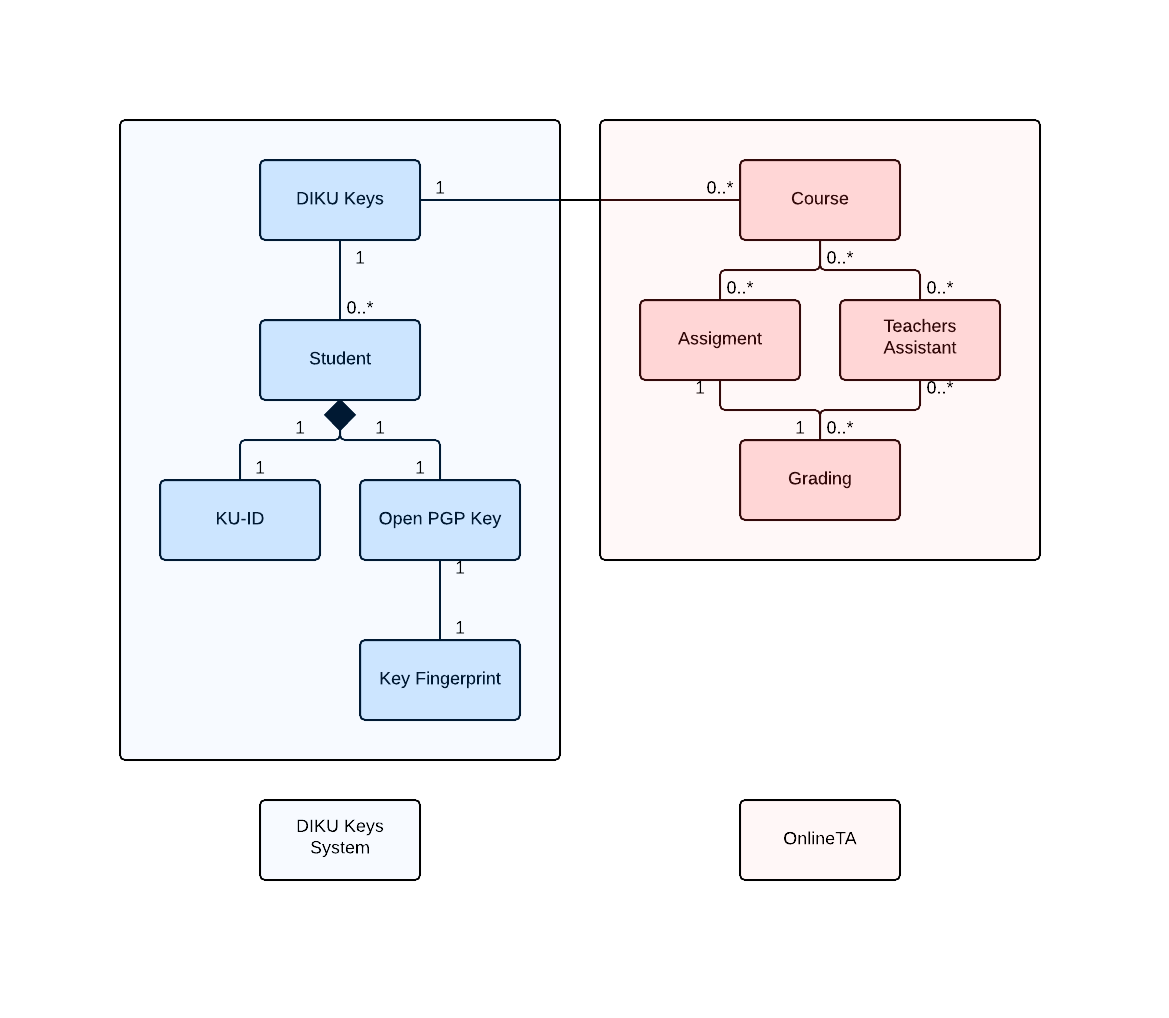
\includegraphics[width=\textwidth]{pictures/class_diagram_v3}
    \caption{Class diagram of solution domain. The DIKU Keys system interacts with grading, courses, assignments, students, public keys, and KU IDs. A few other classes such as course director could also have been added but in this drawing course directors should be viewed as part of the TAs or part of the course. Each student is assumed to have exactly one OpenPGP Key and one KU ID.}
    \label{fig:class_diagram_v3}
\end{figure}
\subsection{BCE Classes}\label{subsec:BCE}
Classes for the system design are defined according to the BCE scheme. This divides the classes into Boundary, Control, and Entity classes. The Boundary classes are the parts of the system with which the end-user interacts, the control classes define the logical operations of the system, and the entity store the persistent states of the system. The boundary classes are identified as the HTML serving which occurs through the webserver and the email server, the control classes are different forms of logic: hash generation generated from KU ID, timestamp, and padding; validation of the uploaded public key; and URL handling which verifies that the GET request contains a valid hash. The entity classes are the mappings which the end-users store: KU ID and public keys.


\begin{center}
\begin{table}[h]
\centering
\begin{tabular}{|l|l|l|}
\hline
\textbf{Boundary}     & \textbf{Control}                  & \textbf{Entity}     \\ \hline
Web server   & Hash generation          & KU ID      \\
Email server & Validation of public key & Public key \\
             & URL parsing              &            \\ \hline
\end{tabular}
\caption{Boundary, control and entity classes for the system.}
\end{table}
\end{center}

%The BCE model is shown in Figure \ref{fig:bce_model}. The BCE model is the \nth{1} attempt to describe the actual system (AKA application) domain since the previous class diagram was of the solution domain. The entitiy classes hold the data stored in the system, the control classes describe the logic of the system, and the boundary classes describe the part of the system that interacts with the end-users: the website and the email system. TA API could also be included here. Two models for the control classes have been described as a final choice has not been made yet.



\subsection{Sequence Diagrams of Use Case}\label{subsec:Sequence_diagram_Use_case_model}
Figure \ref{fig:sequence_diagram} shows the logical flow between the classes identified in the BCE analysis in Section \ref{subsec:BCE}.
\begin{figure}[H]
    \centering
    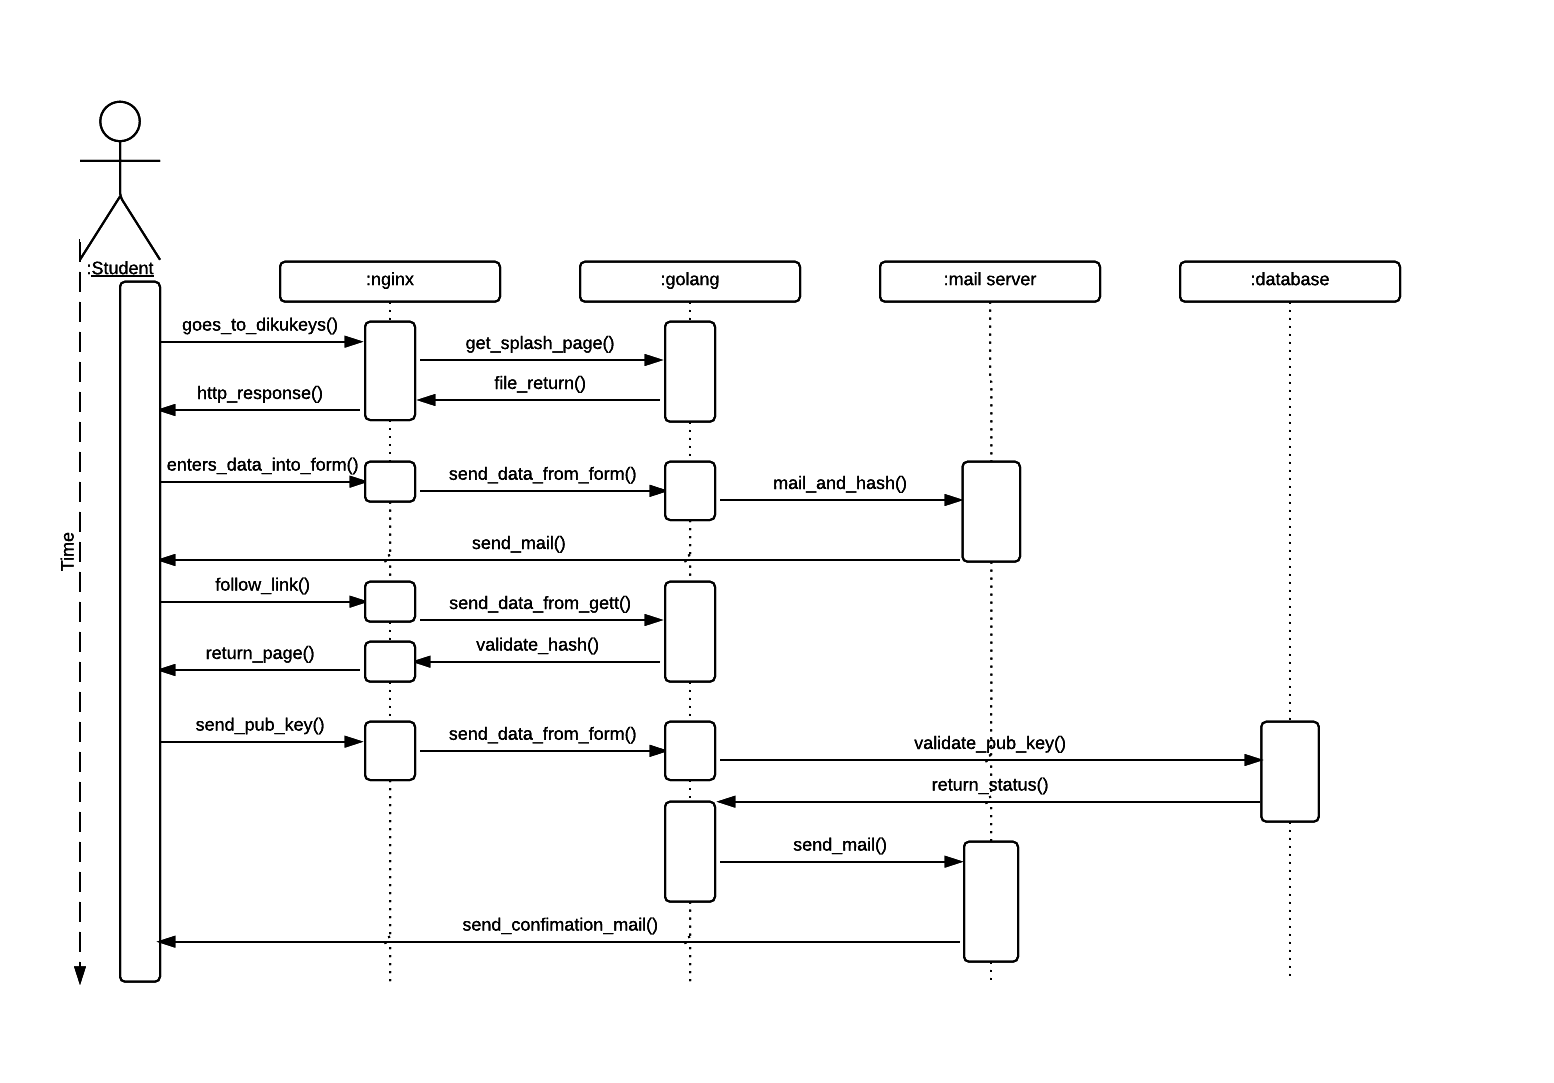
\includegraphics[width=\textwidth]{pictures/sequence_diagram_upload_key}
    \caption{The sequence diagram for the uploading of a public key to the database. Only the boundary classes interact with the user and only the entity class (the database) can permanently change the state of the system.}
    \label{fig:sequence_diagram}
\end{figure}

The sequence diagram for the replacement of a key is practically similar to that of the uploading of a key. Only one function is different: send\_mail() has been replaced by send\_replace\_mail(). Nonetheless, the sequence diagram of that process is presented below.

%In figure \ref{fig:use_case_diagram_example_two} we have modeled the more specific use case for uploading a key.

\begin{figure}[H]
    \centering
    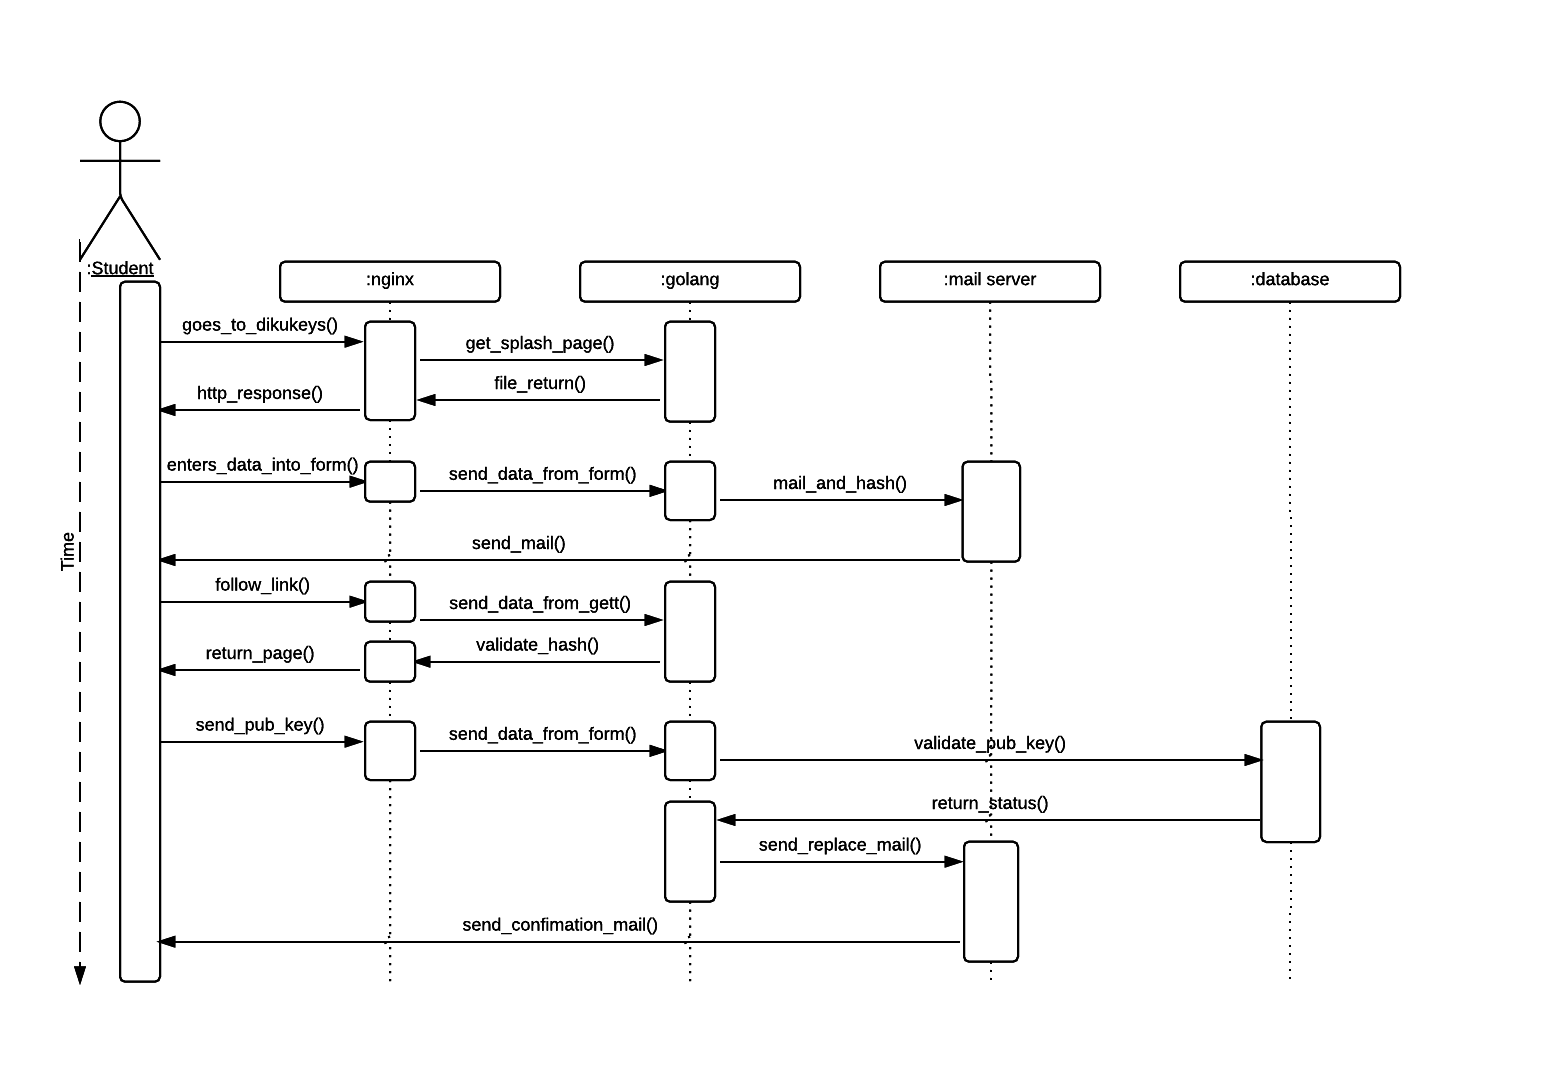
\includegraphics[width=\textwidth]{pictures/sequence_diagram_replace_key}
     \caption{The sequence diagram for the replacement of a public key on the database. Similar to upload of a key but send\_mail() has been replaced by send\_replace\_mail().}
    \label{fig:use_case_diagram_example_two}
\end{figure}

\section{Resumé of System Design}\label{sec:Systemdesign}
\subsection{Implemented Functions}
The system is capable of serving websites to users which are generated by the back-end. This is implemented with nginx as the HTTP-server, FastCGI as the internal communication protocol, and the back-end is written in golang.

The layout of the served websites is adaptive to display size and resolution. This adaptiveness is achieved by using bootstrap. \\
\subsection{Functions not Implemented yet}
There are still core functions which need to be implemented. These are the ability to save data by writing to a database and providing access to the data through an API. Automatic change of the private padding in the hash needs to implemented as well. \\
There are some non-critical functions which need to be implemented as well:
\begin{itemize}
    \item Accepting lists of students in csv-files
    \item Providing manual access to the data to privileged users in some way
    \item Facilitating easy translation by exporting all strings into an external file from which the strings are loaded.
\end{itemize}
Last but not least the system needs to move from a development environment to a production environment which includes end-to-end encryption where possible within reasonable bounds.

\section{Program- and System Tests}\label{sec:Program_systemtests}
We plan to test the system from multiple vectors:
\subsection{Independent Code Review}
To avoid typical pitfalls and errors due to oversight or coding style our code is reviewed by multiple parts. Exceptionally the customer is one of these reviewers and they are quite good at filing bug reports through GitHub.
 When an issue has been raised, it can be assigned to any team member. This will usually be the team member whose skill set matches the issue at hand best.
\subsection{Security Testing}

The hacker group pwnies\footnote{\href{https://pwnies.dk/}{pwnies.dk/}} has been added to our git repository. This will allow them to follow our project and assess vulnerabilities as  we implement the rest of the system. Before reaching release phase, pwnies will perform penetration testing on the system. This will not be done within the regime of the ProjDat course, as our product will not reach production state before the course is concluded. We plan on continuing to work on the project afterwards.\cite{wiki:sectest}

\subsection{Usability testing}
We are in the very fortunate position that we work at the same place of our target group, this allows us to do Hallway testing exceptionally easy. These tests have already aided in the interface design process. See Section \ref{sec:youtube}.% Om folk forstod at skrive sin KU-ID korrekt ind.

\subsection{Unit Testing}
We plan on writing unit tests for all functions in our code, but at the moment this is out of the scope of our time resources. In other words, this is planned to be done some time after the course ProjDat has been concluded.

\subsection{System testing}
We will unfortunately not be able to perform system tests since our subsystem will be the first part of the system to be created.

\newpage
\section{User Interface and Interaction Design}\label{sec:UI_interactiondesign}
\subsection{Screenshots}

The Figure \ref{fig:ss_kuid} shows the initial view a user is met with. It has a fairly simple interface with a form for inputting the user's KU ID and a submit button which should be clicked on to get to the next view. \\

\begin{figure}[H]
\centering
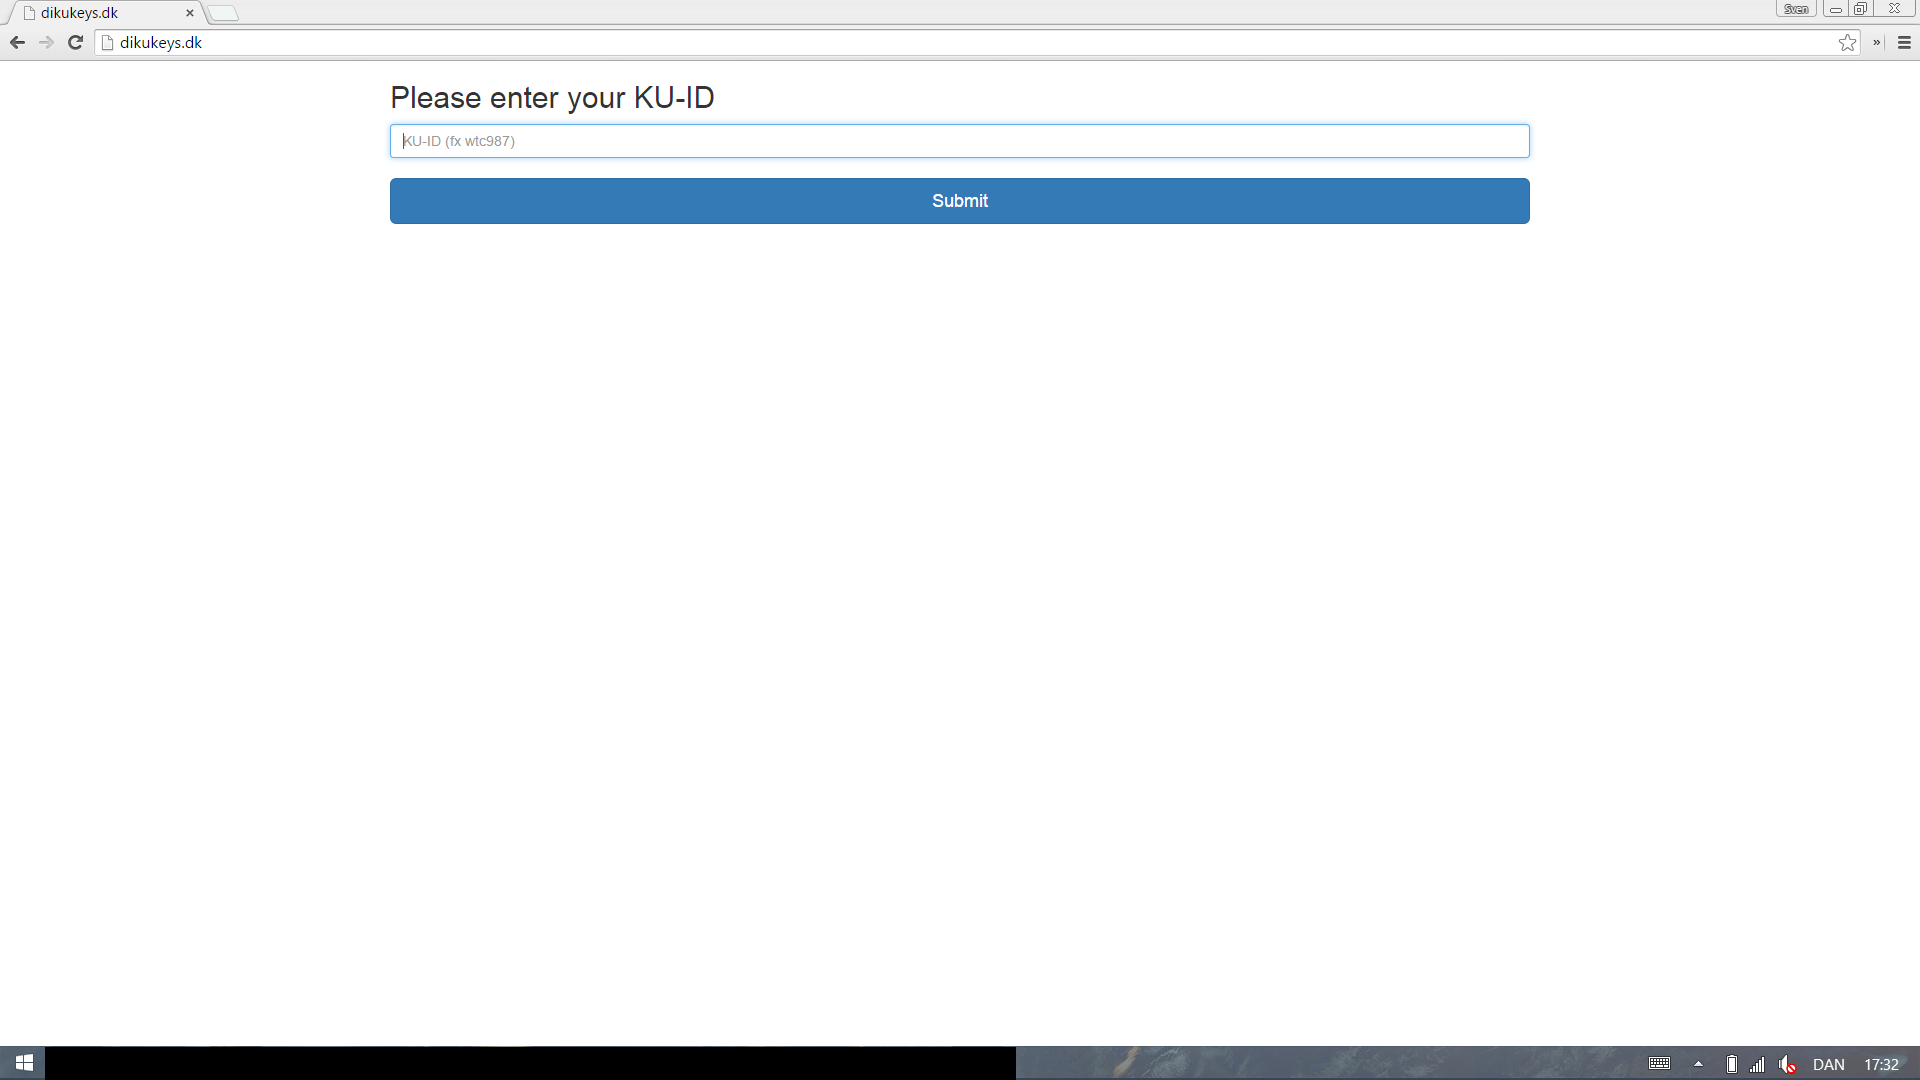
\includegraphics[width=0.9\textwidth]{pictures/screenshots/kuid}
\caption{Landing page on dikukeys.dk. This is where the user enters their KU ID.}
\label{fig:ss_kuid}
\end{figure}
The Figure \ref{fig:ss_email} shows the interface for KU's webmail. The interesting part here is the focused email which is generated when the user clicks on the submit button in Figure \ref{fig:ss_kuid}. \\
The link in the email leads to Figure \ref{fig:ss_pubkey}.\\
\begin{figure}[H]
\centering
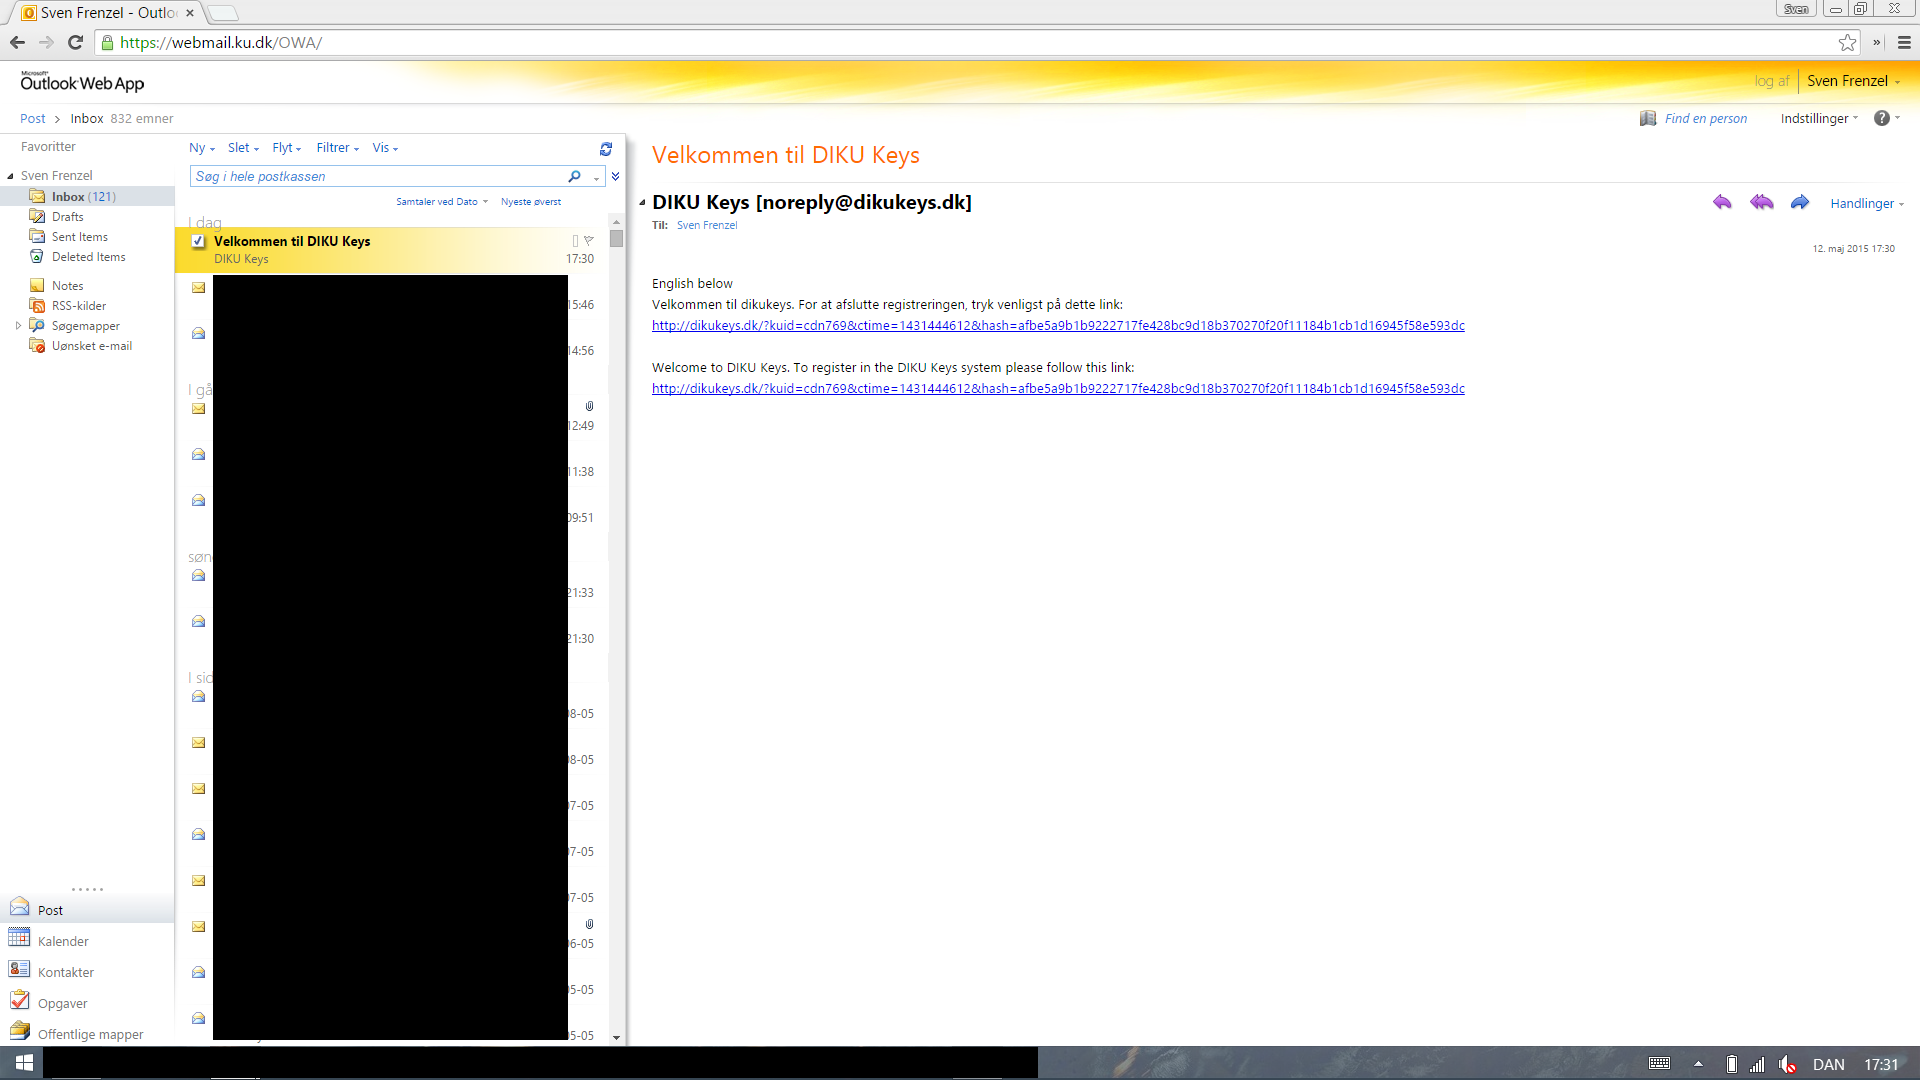
\includegraphics[width=0.9\textwidth]{pictures/screenshots/email}
\caption{The webmail interface of KU. The registration email has been received by the user.}
\label{fig:ss_email}
\end{figure}
Figure \ref{fig:ss_pubkey} shows the interface for submitting a public key. There is a large input field for inserting the users public key and a submit button which will trigger the registration of the user in the system when clicked.
\begin{figure}[H]
\centering
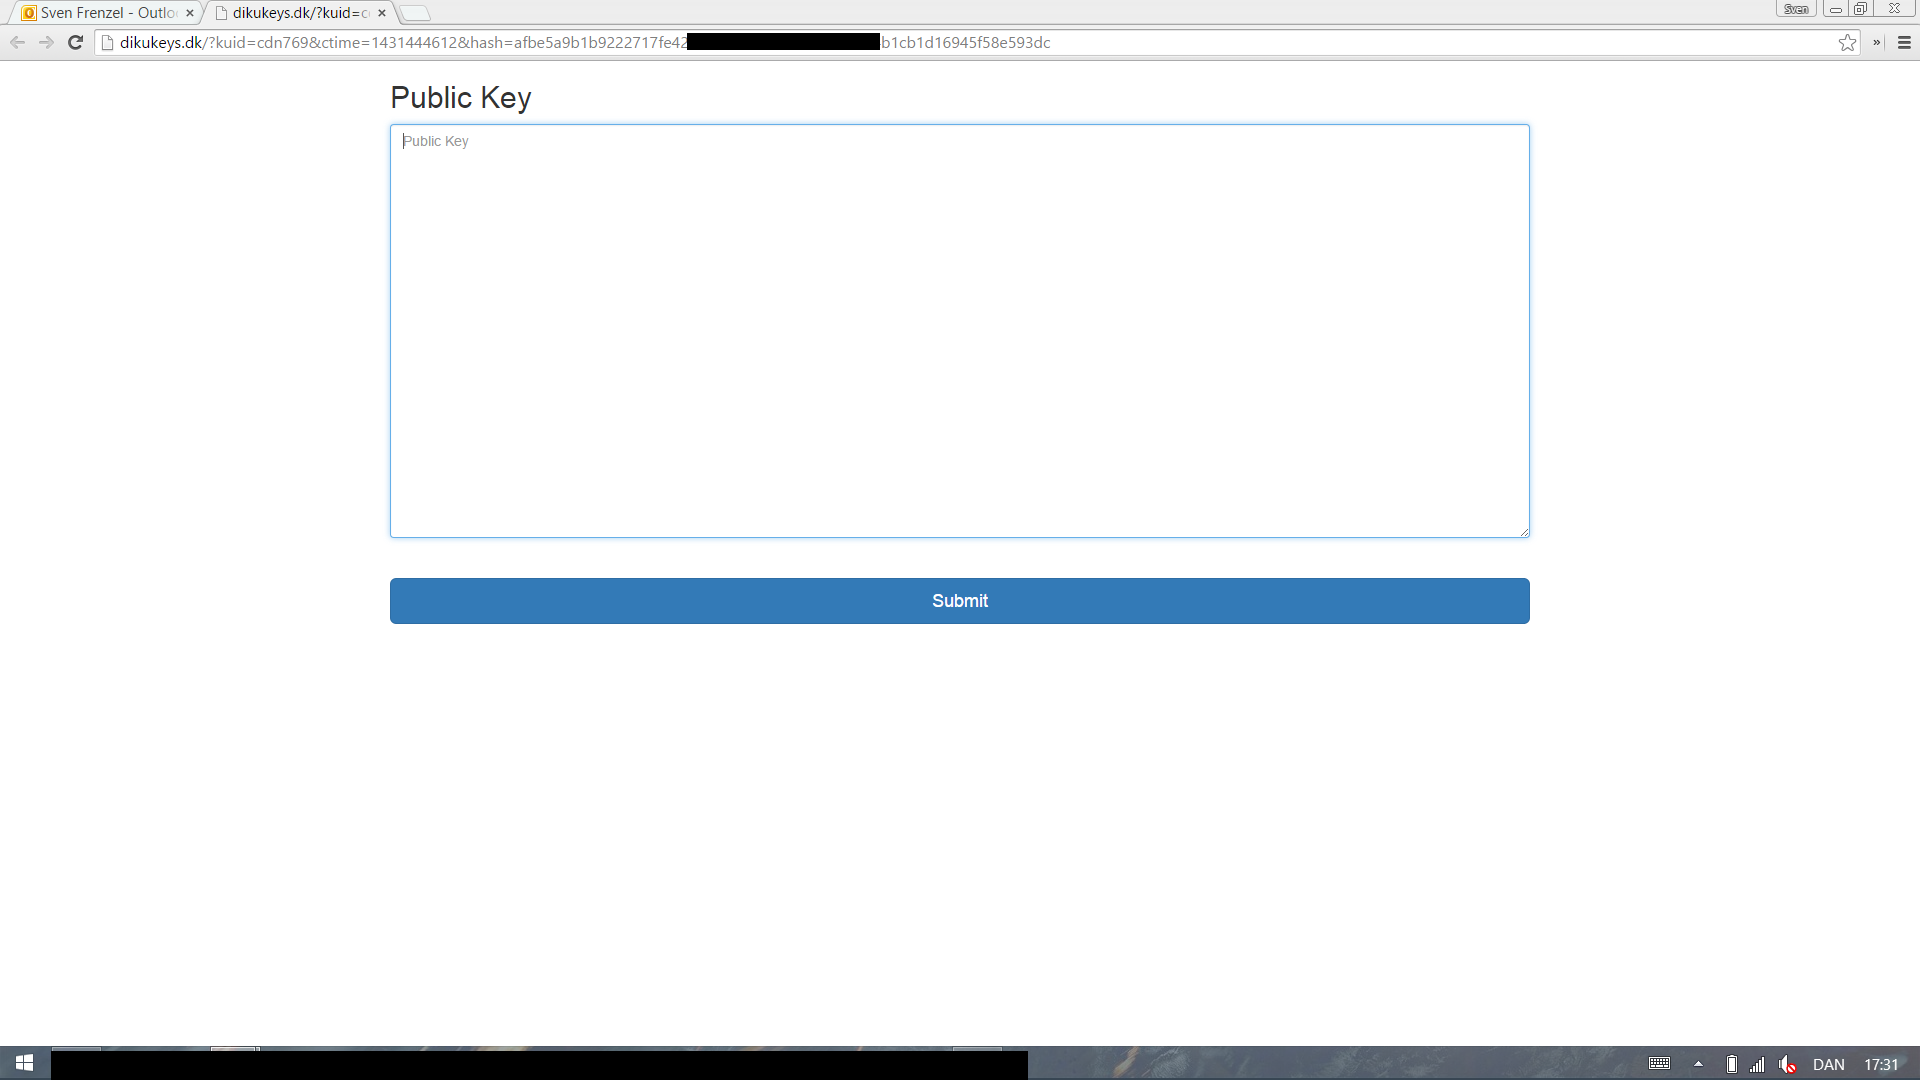
\includegraphics[width=0.9\textwidth]{pictures/screenshots/publickey}
\caption{Page where the user submits their public key. This link is sent in the email above.}
\label{fig:ss_pubkey}
\end{figure}

\subsection{Flow and Dynamics}

\begin{figure}[H]
    \centering
    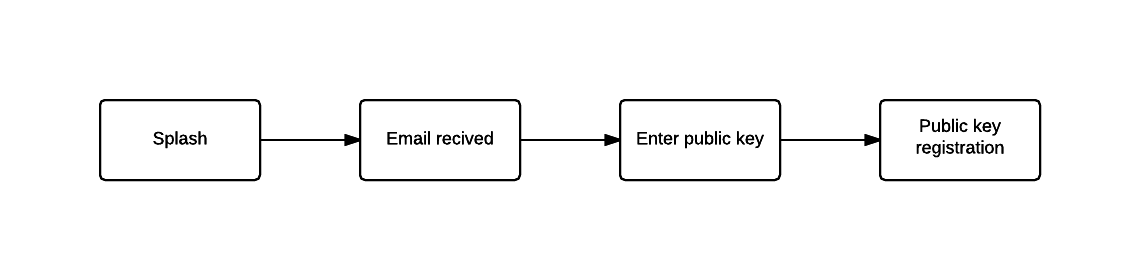
\includegraphics[width=1\textwidth]{pictures/flow_diagram}
    \caption{The flow of interfaces shown to an end-user.}
    \label{fig:flow_diagram}
\end{figure}


\subsection{Audio/Visual presentation} \label{sec:youtube}

A screen cast of Sven Frenzel using the system is available at \href{https://youtu.be/lKnijMJSObA}{https://youtu.be/lKnijMJSObA}. It walks through all the necessary steps to register with DIKU Keys, but omits the process of creating an OpenPGP key pair.
\subsection{Think Aloud User Test}

A think aloud test was performed on a person that had heard about the system but not used it before. A short introduction was given to the user and he was asked to access the website and follow the steps.

The user managed to enter his KU ID, receive the mail, press the link in the mail, and enter a public key. Some guidance was given to help him upload a public key since he was not familiar with the operating system's (Windows 8) key handling. He provided the following feedback.
\begin{itemize}
    \item The splash screen contained too little information. A short explanation was requested.
    \item He would like to have a green light/green text -- implementable through JavaScript -- indicating that a correct public key was entered.
    \item A short text in the email saying that this email can be ignored if the KU user has not asked to be registered in the system.
    \item It would be easier to upload a public key if an option was given to upload an entire text file. Right now, you have to paste the text into a text field in the website.
\end{itemize}
We did not find time to implement these changes but they are provided for reference to future work.


\section{Group Dynamics}
\subsection{What is Good?}
The knowledge level of the group seems high considering that we are \nth{1} year students. The group members complement each other well since Sven Frenzel is a smart and fast learner with an eye for detail, especially when it comes to the logic of systems. Frenzel has undertaken the vast majority of the server configuration. Mads Gram has a lot of knowledge in web-design and developing websites, in addition he has made most of the technical diagrams such as the class diagram and the sequence diagrams. Thorkil Værge has a good overview and often delegates work, while still doing a significant amount of the textual work, since his written English is remarkable.

Since the talents of the group are varied we are able to approach the subject from many different perspectives.

The company and social dynamics in the group are pleasant. We work very well when we are brainstorming and dividing up the work amongst ourselves.

\subsection{What is Bad?}
Sven can have a difficulty staying focused and have been absent a bit too much. When we work in the canteen of DIKU, he is easily distracted by other students. Thorkil should spend a bit more time on the code since Mads and Sven have spent more time on this than he has. His golang skills are quite good, though.

The work process on the \nth{2} report has not been as good as the process for the \nth{1} report since the group has not met and worked together more than one whole day. The rest of the work has been done individually or in groups of two. A better report would have been made if we had dedicated one more day to this report.

The work process on the \nth{3} report has been fairly good since many of the hard work was done in the \nth{2} report and the resubmission of the \nth{2} report.

Thorkil Værge feels that we use too much time on reports and not enough time on programming and actual systems design. We do, however, learn something from all the different models for the system that we have to make.

\subsection{How can this be improved?}
To improve our work process, we should have more days where we do nothing but work on this project. Experience shows us that these days are the most effective way to work.

Furthermore experience shows that we are most effective when working as a group in a closed meeting room where there are no distraction. We should thus avoid working in the canteen at DIKU.

\newpage
\begin{appendices}
\chapter{Version Control}

We have chosen to use Git as our version control solution, this we have pared with the only git repository host GitHub.

As earlier agreed upon with our instructor Kasper Passov, we have added him to our Git repository. This will allow him to access our source code.

<<<<<<< HEAD
\href{https://github.com/Orkeren/DIKU-Keyserver/commit/5e7c7c741fbe6d2e74889e8eaff6173e8c116d46}{\textbf{Inital commit on github.}}
=======
\href{https://github.com/Orkeren/DIKU-Keyserver/commit/5e7c7c741fbe6d2e74889e8eaff6173e8c116d46}{Inital commit on GitHub.}
>>>>>>> 1a2fe1ffd3be8f658cef3d9e3a8684031a70ec1d

This is the initial commit with focus on our source code. It is divided into three parts, app, hash, and mail. App.go is the overarching module, which controls the web-application, the function of App.go is to interface with the web-server (nginx) and the other modules.

hash.go is a go module which enables creation of cryptographic hashes, in this iteration of the code, we only printed it to the console.  The file mail.go is another module which the code uses, this is used to send out mails, in this iteration we used it to send out a mail to our dikumail group, to show how far we were.

<<<<<<< HEAD
\href{https://github.com/Orkeren/DIKU-Keyserver/commit/690f4b0b00dc68e9b529035d7e6e6a6005072d63}{\textbf{Using HTML templates commit on github.}}
=======
\href{https://github.com/Orkeren/DIKU-Keyserver/commit/690f4b0b00dc68e9b529035d7e6e6a6005072d63}{Using HTML templates commit on GitHub.}
>>>>>>> 1a2fe1ffd3be8f658cef3d9e3a8684031a70ec1d

Earlier we used pre-encoded HTML in our app.go, with modification and extensive use of the html/template library. We were able to use html templates rather. This allows us to make changes to the pages which are displayed, without stopping the service.


\href{https://github.com/Orkeren/DIKU-Keyserver/commit/78fd1efa312d4022ecb66a13c0614069a4ff094c}{\textbf{Add from and subject to mail}}

In this commit, we added a subject field and a from field in the emails sent by the system. This ensured that our mails were no longer caught by Office 365's spam filter. This spam filter caught all mails sent to KU users since the KU uses Microsoft's email system.

\href{https://github.com/Orkeren/DIKU-Keyserver/commit/09610ad45946dddbcf73c5db870eae36a591e0ef}{\textbf{Added regular expression}}

Added regular expression checks on the backend so the users can only send valid KU IDs to the server (three consonants and three decimal digits). This check also exists on the front-end in the form of a Javascript.

\href{https://github.com/Orkeren/DIKU-Keyserver/commit/a75d93cb59f7c662260f76104f2bb739c9390fce}{\textbf{Changed hash length after meeting with client}}

The client thought that the validation hash links sent in the emails were too long. So the hashing algorithm was changed from SHA512 to SHA256.

\chapter{Changelog for report}

Since we use Git for our entire project, a timeline of a specific file is possible, so for our report the timeline consists of a link to a history of our document, which our document has been built from. Since we all have individual GitHub accounts, it is possible to see who committed what.

\href{https://github.com/Orkeren/DIKU-Keyserver/commits/master/docs/delrapport_2/aflevering2.tex}{Aflevering2.tex on GitHub.}


\chapter{Timeline}
\begin{itemize}
  \item  March 16th 2015: First meeting with client, initial establishment of project. We agreed upon programming language and choice for authentication Open-PGP keys.
  \item  March 22th 2015: Second meeting with client, here we went into specifics alike API for staff and license
  \item March 29th 2015: Third meeting with client, we agreed upon using nginx as our webserver and some discussion about which database was started, but a final agreement was not reached. Lastly we agreed upon using the Bootstrap framework for the front end design. We setup a test server the same day, and got our first prototype ready.
\end{itemize}

\chapter{Minutes}
\section{Minutes from March \nth{16} 2015}
\begin{itemize}
\item Ønsker: identificer studerende ved aflevering vha gpg-nøgle
\item Ønsker: grube med gpg-nøgle og ku-mail knyttet sammen (da der stoles på at den studerende har adgang til sin email)
\item Autentificering sker igennem unikke links til ku-mail (for at lægge gpg-nøgle op).
\SubItem 2 muligheder: copy/paste gpg-nøgle eller generer gpg-nøglepar direkte i browseren.
\item DIKU leverer ssl-certifikat.
\item Hvorfor ikke bruge eksisterende?
\item Public index j/n?
\item modtager ukrypteret nøgle og bruger den til at verificere indholdet - bagefter checkes hashet pubkey mod databasen.
\item Arbejdsbelastning: 10 timer per person per uger
\item database: (\underline{ku-nummerplade},hash(pubkey))
\end{itemize}
\subsubsection{Krav:}
\begin{itemize}
\item registrering gennem webformular og/eller kommandelinje
\item skal kunne genregistrering
\item anmodning kodkendes igennem KU email
\item kunne vælge om den offentlige nøgle offentliggøres
\SubItem private by default
\item private API: få offentlig nøgle og returner brugernavn (kun adgang til DIKU-ansatte)
\item Sprog
\SubItem Backend: golang + sql
\SubItem frontend: html5 + js
\end{itemize}

næste møde:
2015-03-22 kl 11-16

\section{Minutes from March \nth{22} 2015}
The meeting was held to align the expectations of the client and the developers in regards to the systems capabilities and design.

\begin{itemize}
\item Oleks undersøger interface hvilke tilgangsmuligheder, der ønskes til databasen.
\item Kun lukket API, intet offentligt look-up. Der gemmes pupkey og abc123 (ku-brugernavn).
\item key-server i stil med MIT-keyserver er nice-to-have. Man bliver kun listet her, hvis man eksplicit ønsker dette.
\item Den studerende uploader en fil til afleveringssystemet (uden anden information). Afleveringssystemet anmoder om par af PubKey \& KU-ID og undersøger om filen er signeret af denne nøgle. Hvis ikke, så anmodes næste par indtil det korrekte par er fundet. Dette returneres til underviser.
\item Beta klar til start/midt maj.
\item Oleks gives a license (MIT-like)
\item ISA-diagram
\SubItem Fjern Admin-login fra (der er sshd-adgang til serveren anyways.)
\SubItem Front-end til client, er response og ikke request
\SubItem User guide /shell script ved ``Create key''
\item Oleks anmoder om at der sendes en dagsorden 24 timer før fremtidige møder
\item Thorkil foreslår at møder optages auditivt.
\end{itemize}


\section{Minutes from May \nth{5} 2015}

\textbf{Present: Oleksander Shturmov (Client), Sven Frenzel, Mads Gram, and Thorkil Værge }

\begin{itemize}
\item Oleks wants information on the landing page.\\
\item Edit the ku-id check\\
\item After posting a ku-id, the page should return the posted ku-id\\
\item JS regex needs to be updated\\
\item Fix ``å'' in email.\\
\item e-mail in english after the danish paragraph\\
\item More content in the e-mail. Standard ``you cannot reply. if this wasn't you.''\\
\item Shorter hash in link\\
\item More description on pgp-submit page.\\
\item Check if content submitted is an OpenPGP public key.\\
\item Make sure link can be used only once\\
\item Bootstrap change a bit layout\\
\item Streamline language\\
\end{itemize}



\end{appendices}
\nocite{*}

\bibliography{aflevering4}
\bibliographystyle{ieeetr}
\end{document}
